\chapter{Related works}

This chapter presents the related works we started from to develop this work. Firstly we introduce a paper from Laurenza et al. that explain how to build a malware triage for APT classification. The second work, from Caliskan et al., shows how is it possible to de-anonymize different programmers even with a compiled executable. The last work of Dubyk propose an approach for malware similarities based on the Rich Header.

\section{Malware Triage Based on Static Features and Public APT Reports}
Laurenza et al. show that it is possible to help an analyst lightening the number of samples to analyze. They proposed an architecture for sample prioritization, which, based on a rank score, decides which sample has the priority to be further inspected by an analyst. In this way, it is possible to avoid wasting time analyzing samples that are not important. 

They decide to rely only on static analysis instead of dynamic analysis to improve the speed of processing. In this architecture, the time elapsed for analyzing a classifying the samples is more important than the accuracy of the classification. Since it relies on static analysis, there is no need for sample execution, or to set up a complex virtualized environment. Every sample is processed, and some features are extracted from the header. The knowledge base created is used to classify new malware.

\begin{figure}
	\centering
	\begin{subfigure}{1.0\textwidth}
		\centering		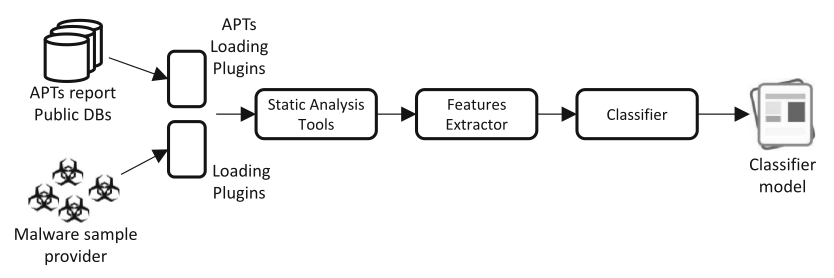
\includegraphics[width=1.0\linewidth]{train.png}  
		\caption{Training phase}
		\label{fig:sub-train}
	\end{subfigure}
	
	\begin{subfigure}{1.0\textwidth}
		\centering
		% include second image
		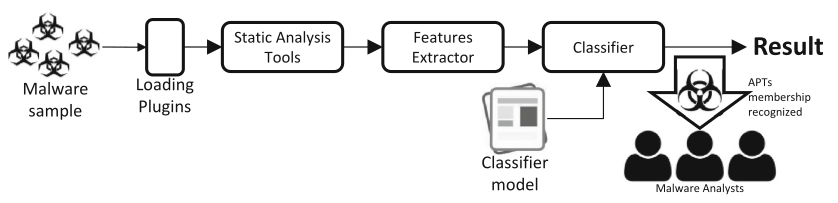
\includegraphics[width=1.0\linewidth]{test.png}  
		\caption{Testing phase}
		\label{fig:sub-test}
	\end{subfigure}
	
	\caption{Malware triage flow.}
	\label{fig:mal_triage}
\end{figure}

They proposed a malware triage architecture, based on the identification of malware similar to other malware known to be related to some APTs campaign. The idea is to collect public APT reports and their related samples.  Then, extracting features from the samples and assigning them to the class of the APT they belong to. Those features vectors are used to train a classifier.



Figure \ref{fig:mal_triage} shows the architecture of both the training and testing phases. The APTs loading plugin frequently loads the information on APT crawled from public reports on the internet. The loading plugin feeds the system with new samples from different sources. The features extraction phase produces the features vectors from the malware, continuously updated by the previous loading plugin. In the classifier phase, a classifier is trained with features vector. 

In the analysis phase, novel samples follow the same pipeline; the features extraction stage extracts the features vector that is passed to the classifier. If the output of the classifier is positive, i.e., the sample is related a know APT, then the sample follows a different path, and is sent a human analyst for further inspection, otherwise it is discarded.

Unfortunately, this work has some drawbacks. First of all, it is possible to identify only samples correlated to a known APT campaign, if the sample belongs to a new never investigated APT, then it is impossible to detect it. Furthermore, even if the executable belongs to a known APT, there is no guarantee that the classifier detects it because it just relies on information present in the header of the file. The malware writer can hijack that information to mislead the model.

\textbf{BOOOO}
\\

The idea in our work is to boost up Laurenza's et al. work, introducing different features without slowing down the entire flow. As written in their future works, they wanted to extend the architecture to new kind of features, based on code analysis. 





The dataset used by Laurenza et al. is \textbf{dAPTaset}, a public database that collects data related to APTs from existing public sources through a semi-automatic methodology and produces an exhaustive dataset. Unfortunately, the dataset is not big enough and is not perfectly balanced. It contains only 2086 samples because there are not many samples belonging to an APT campaign. Instead, the majority of public analyzed samples are just malware.

\section{De-anonymizing Programmers from Executable Binaries}
In this paper, Caliskan et al. presented their approach to de-anonymize different programmers from their compiled programs. They used a dataset of executables from Google Code Jam, and they show that even after compilation the author fingerprints persist in the code, and it is still possible to de-anonymize them.\\

Their approach was to extract distinct blocks of features with different tools and then analyze them to determine the best ones to describe the stylistic fingerprint of the authors precisely. Firstly,  with a disassembler is possible to disassemble the binary and to obtain the low-level features in assembly code.

Then with a decompiler, they extracted the \textbf{Control Flow Graph} and the \textbf{Abstract Syntax Tree}. They determine the stylistics features from those four documents.
\\
In particular, the tools used are \textbf{ndisasm} \textbf{radare2} disassembler for the disassembled code and the Control Flow Graph; \textbf{Hexray} decompiler for the pseudocode, which is passed as input to \textbf{Joern}, a C fuzzy parser, to produce the  \textbf{Abstract Syntax Tree}.\\

They used different types of features selection techniques to reduce the number of features to only 53. They trained a RandomForest Classifier with the dataset created to de-anonymize the authors correctly. \\

This paper is an entry point for our work, and we tried to apply the same approach to the apt triage problem. However, the tools used by Caliskan et al. are outdated and no more maintained, so we decided to use the novel open-source tool ghidra to write the script and extract the information we want. In this way, we significantly reduced the amount of time for feature extraction.



\section{Rich Header}

The work of Maksim Dubyk \cite{dubyk2019sans} shows how the rich header produces a robust series of data points that can be exploited in static PE-based malware detection. The Rich Header is an undocumented section of \textit{Portable Executable} (\textbf{PE}) header and provides a view of the environment where the executable was built. Firstly, Dubik shows the location of the Rich Header, how to understand and decrypt it, and how to extract it. Then, he shows different techniques to leverage the header for PE-based malware classification. The Rich Header is part of our features vector.

When building a PE, there are two distinct phases. The first one is the \textit{compilation phase}, where the high-level instructions from programming language are compiled into machine code, executable by the computer. The second one is the \textit{linking phase},a combination of those different machine code objects into a single executable. The act of combining different objects creates the Rich Header. However, only executables compiled with Microsoft Linker contain the rich header, other compilers, such as gcc or .Net,  do not have it.

\begin{figure}[!h]
	\centering
	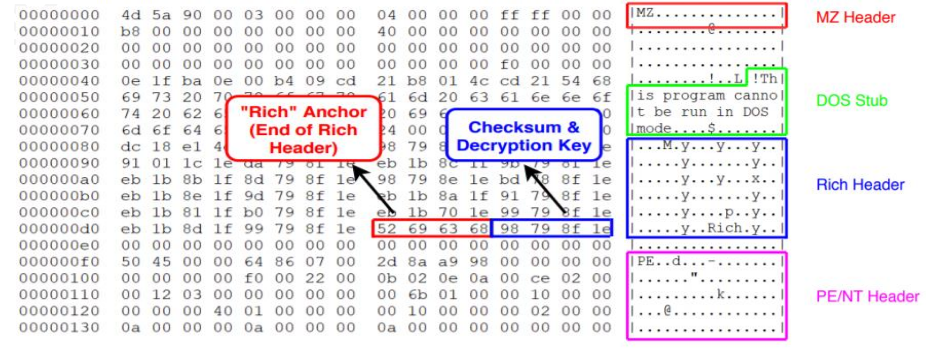
\includegraphics[width=1.0\columnwidth]{cmd.png}
	\caption{Hexview of cmd.exe}
	\label{fig:cmd}
\end{figure}

Analyzing an executable with a hexdump, the Rich Header starts from location \texttt{0x80} until the bytes sequence \texttt{0x52696368}, which means \textbf{"Rich"} in ASCII. Figure \ref{fig:cmd} shows the location of Rich header and the ending string "Rich". The content of the rich header is encrypted, and the corresponding decryption key and checksum are located right after the "Rich" string. 

The algorithm that computes the decryption key takes advantage of two checksum algorithms. The first checksum is generated from the bytes that make the DOS header, but with the \texttt{e\_lfanew} field zeroed out\cite{richHeaderHunting}. The second checksum is the combination of each value in the array generated. The outputs of the checksum algorithms are summed together and then masked with the bytes \texttt{0xFFFFFFF}, the key generated is then used to encrypt the rich header section using the XOR.

It is straightforward to decrypt the rich header section. The key found after the "Rich" string is XORed backward with the chunks of the section until the end string "DanS" is found.  

The decrypted rich header is an array that stores metadata related to each phase of the linking process. Each array's element is an 8-byte structure that contains three fields: \textit{product identification} (\textbf{pID}), \textit{product version} (\textbf{pV}), and a \textit{product count} (\textbf{pC}). Those numbers identify the Microsoft product used in that linking phase. However, since the Rich Header is an undocumented section, there is no official mapping of pID with Microsoft products. Nevertheless, some researches partially mapped out some pID with known compilers \cite{richGit}.

To calculate the rich header of each sample, we used the python script provided in \cite{dubyk2019sans}.


\section{Advanced Persistent Threat}

APT stands for Advanced Persistent Threat, a kind of sophisticated attack which requires an advanced level of expertise and aims to remain persistent on the attacked infrastructure.

The term APT can refer to a persistent attack with a specific target, or it can refer to the group that organized the attack, sometimes the group is affiliated with some sovereign state.
\\

To understand better what is an APT, we need to decompose the word: 

\textbf{Advanced:} the people behind the attack have an advanced level of expertise, resources, and money. They usually do not use known malware, but they write their malware specific to the target they want. Moreover, they can gather information on the target from the intelligence of their country of origin.

\textbf{Persistent:}  The adversary does not aim to gain access in the most number of system, but rather to have persistent access to the infrastructure. The more time they remain undiscovered in the organization's network infrastructure, the higher are the chances of lateral movement, the greater are the information they can gather. Persistent access is the key to every APT.

\textbf{Threat:} As said before, this is an organized threat, with a strategical vision of what to achieve. It is not an automatic tool that attacks everything trying to gather something. It is a meticulously planned attack that aims to obtain certain information from a given organization. \cite{apt_def}
\\

In general, APTs aim to higher-value targets like other nations or some big corporations. However, any individual can be a target. FireEye publish a report each year about the new APT campaign, the diagram below states which industry is the most attacked in the last year.\\

\begin{figure}[!h]
	\centering
	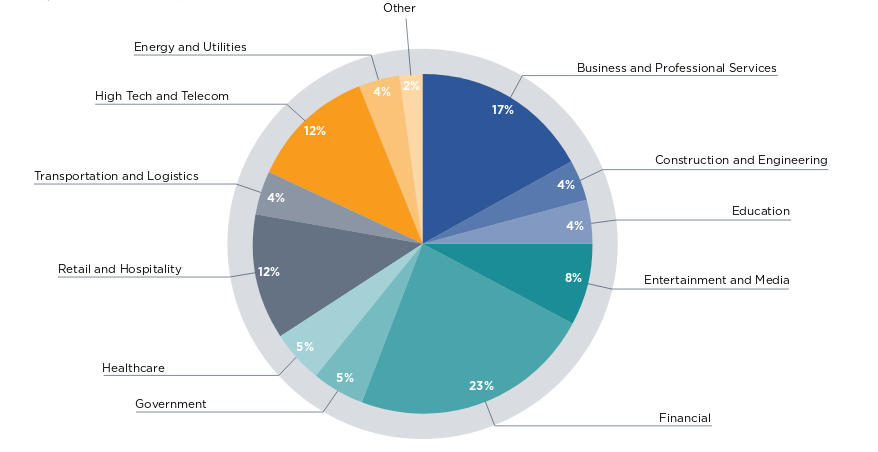
\includegraphics[width=1.0\columnwidth]{graph}
	\caption{Diagram of industry target}
\end{figure}

A point of particular concern is the retargeting, in the Americas, 63\% of the companies attacked by an APT, are attacked again last year by the same or similar group. In the Asian and Pacific areas, this is even worse, 78\% of the industries are hacked again. \cite{fireeye_mtrends} \\


\begin{figure}[ht!]
	\centering
	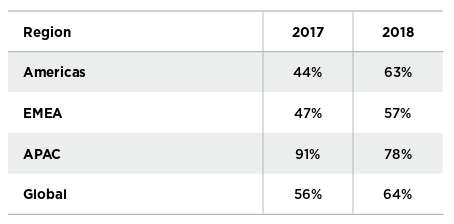
\includegraphics[width=0.5\columnwidth]{retarget}
	\caption{Retargeting divided by regions}
\end{figure}

Advanced persistent threats, contrary to regular malware, are composed of different phases, each of which has an important role. 

The attack is decomposed into smaller steps, for example, if a group of hackers wants to attack a CEO of a given company, they will not send directly to the CEO a phishing email, because it's likely that he has a complex system of security and they would be detected instantly. 

Instead, the first step would hack a person in the same company with lower permissions that can have minor defense mechanisms. Once they got the first computer, they can explore the network infrastructure of the organization, and then decide which action is the best.
They could cover their track from the log system, or locate the data they need or send a phishing email to the CEO from the owned user.\\

So how does an APT work? Fireeye described their behavior in six steps. \cite{fireeye_anatomy}


\begin{enumerate}
	\item The adversary gains access into the network infrastructure, installing a malware sent through a phishing email or by exploiting some vulnerability.
	\item Once they comprised the network, the malware scans all the infrastructure looking for other entry points or weaknesses. It can communicate with a Command \& Control server (C\&C) to receive new instructions or to send information.
	\item The malware typically establishes additional points of compromise to ensure that the attack can continue even if a position is closed.
	\item Once the attackers have a reliable connection to the network, they start dumping data such as usernames and passwords, to gain credentials.
	
	\item The malware sends the data to a server where the attackers can receive the information. Now the network is breached.
	
	\item The malware tries to cover its tracks cleaning the log system, but the network is still compromised so the adversary can enter again if they are not detected.
	
\end{enumerate}